%%%%%%%%%%%%%%%%%%%%%%%%%%EJERCICIO 8c %%%%%%%%%%%%%%%%%%%%%%%%%%%
    \textbf{Solución c.}\\
	%La tabla ira centrada
	\begin{center}
		\renewcommand{\arraystretch}{1.5}% Margenes de las celdas
		%Creación de la cuadricula de 3 columnas
		\begin{longtable}[H]{|p{0.5\linewidth}|p{0.5\linewidth}|}
			%Creamos una linea horizontal
			\hline
			%Definimos el color de la primera fila
			\rowcolor[HTML]{FFB183}
			%%%%% INICIO ASIGNACIÓN FECHA FOCAL %%%%%%%
			%%%%%%%%%% INICIO TITULO
			%Lo que se hace aquí es mezclar las 3 columnas en una sola
			\multicolumn{2}{|c|}{\cellcolor[HTML]{FFB183}\textbf{1. Asignación período focal}}   \\ \hline
			%%%%%%%%%% FIN TITULO
			%%%%% INICIO DECLARACIÓN DE VARIABLES %%%%%%%
			\multicolumn{2}{|c|}{$pf = 0 \textit{ psv}$}\\ \hline
			%%%%%%%%%% INICIO TITULO
			%Lo que se hace aquí es mezclar las 3 columnas en una sola
			\multicolumn{2}{|c|}{\cellcolor[HTML]{FFB183}\textbf{2. Declaración de variables}}   \\ \hline
			%%%%%%%%%% FIN TITULO
			%%%%%%%%%% INICIO DE MATEMÁTICAS
			%Cada & hace referencia al paso de la siguiente columna
			$m =2  \hspace{1mm} psv $  				& $g =25\%  $  \\
			$i = 16\%  \hspace{1mm} psv$      	    & $n=3 \hspace{1mm} pav $ \\
			$ $          			                & $i\equiv 34,56\%  \hspace{1mm} pav$ \\ \hline
			%%%%%%%%%% FIN DE MATEMÁTICAS
			%%%%% FIN DECLARACIÓN DE VARIABLES
			
			\rowcolor[HTML]{FFB183}
			\multicolumn{2}{|c|}{\cellcolor[HTML]{FFB183}\textbf{3. Diagrama de flujo de caja}} \\ \hline
			\multicolumn{2}{|c|}{ 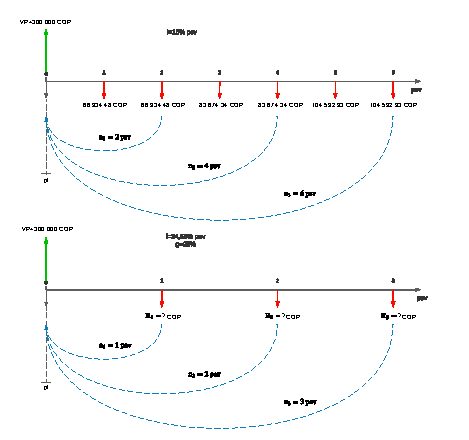
\includegraphics[trim=-78 -5 -78 -5]{7_Capitulo/img/ejemplos/8/8_3.pdf} }   \\ \hline
			%%%%% INICIO FLUJO DE CAJA
			\rowcolor[HTML]{FFB183}
			\multicolumn{2}{|c|}{\cellcolor[HTML]{FFB183}\textbf{4. Declaración de fórmulas}} \\ \hline
			%%%%%%%%%%%%% FIN INSERCIÓN DE IMAGEN
			%%%%%FIN FLUJO DE CAJA
		
			\multicolumn{2}{|c|}{ $VP = \frac{R( (1 + g)^{n} (1+i)^{-n} - 1)}{g-i} $ Valor presente gradiente geométrico}   \\  \hline
			
			%%%%%% INICIO DESARROLLO MATEMÁTICO
			\rowcolor[HTML]{FFB183}
			%%%%%%%%%%INICIO TITULO
			\multicolumn{2}{|c|}{\cellcolor[HTML]{FFB183}\textbf{5. Desarrollo matemático}}       \\ \hline
			%%%%%%%%%% FIN TITULO
			%%%%%%%%%% INICIO MATEMÁTICAS
			\multicolumn{2}{|c|}{  $300.000 \ COP = \frac{R_{1}( (1 + 0,25)^{3} (1+0,3456)^{-3} - 1)}{0,25-0,3456} $}   \\ 
			\multicolumn{2}{|c|}{ $ R_{1} = 225.920,73 \ COP $ }   \\ \hline
			
			%%%%%%%%%% FIN MATEMÁTICAS
			%%%%%% FIN DESARROLLO MATEMÁTICO
			%%%%%% INICIO RESPUESTA
			\rowcolor[HTML]{FFB183}
			%%%%%%%%%%INICIO TITULO
			\multicolumn{2}{|c|}{\cellcolor[HTML]{FFB183}\textbf{6. Respuesta}}   \\ \hline
			%%%%%%%%%% FIN TITULO
			%%%%%%%%%% INICIO RESPUESTA MATEMÁTICA
			\multicolumn{2}{|c|}{ 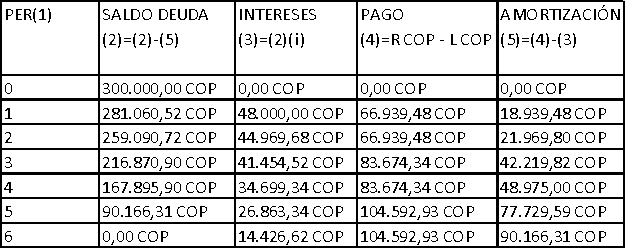
\includegraphics[trim=-78 -5 -78 -5]{7_Capitulo/img/ejemplos/8/8_3_3.pdf} }   \\ \hline
			%\multicolumn{2}{|C{\textwidth}|}{
			%	$R_{58} =  COP  72.478,16(1 + 0,02)^{57} =  COP  224.087,15 $ 
			%}  \\ \hline
			
			
			%%%%%%%%%% FIN MATEMÁTICAS
			%%%%%% FIN RESPUESTA
		\end{longtable}
		%Se crean dos lineas en blanco para que no quede el siguiente texto tan pegado
		%\newline \newline %USARLO SI CREES QUE ES NECESARIO
	\end{center}
 %%%%%%%%%%%%%%%%%%%%%%%%%%FIN EJERCICIO 8c %%%%%%%%%%%%%%%%%%%%%%%%%%%